\chapter{Realisierter Entwurf}
\section{altes Klassendiagramm}
\\[\intextsep]
\begin{minipage}{\linewidth}
\centering%
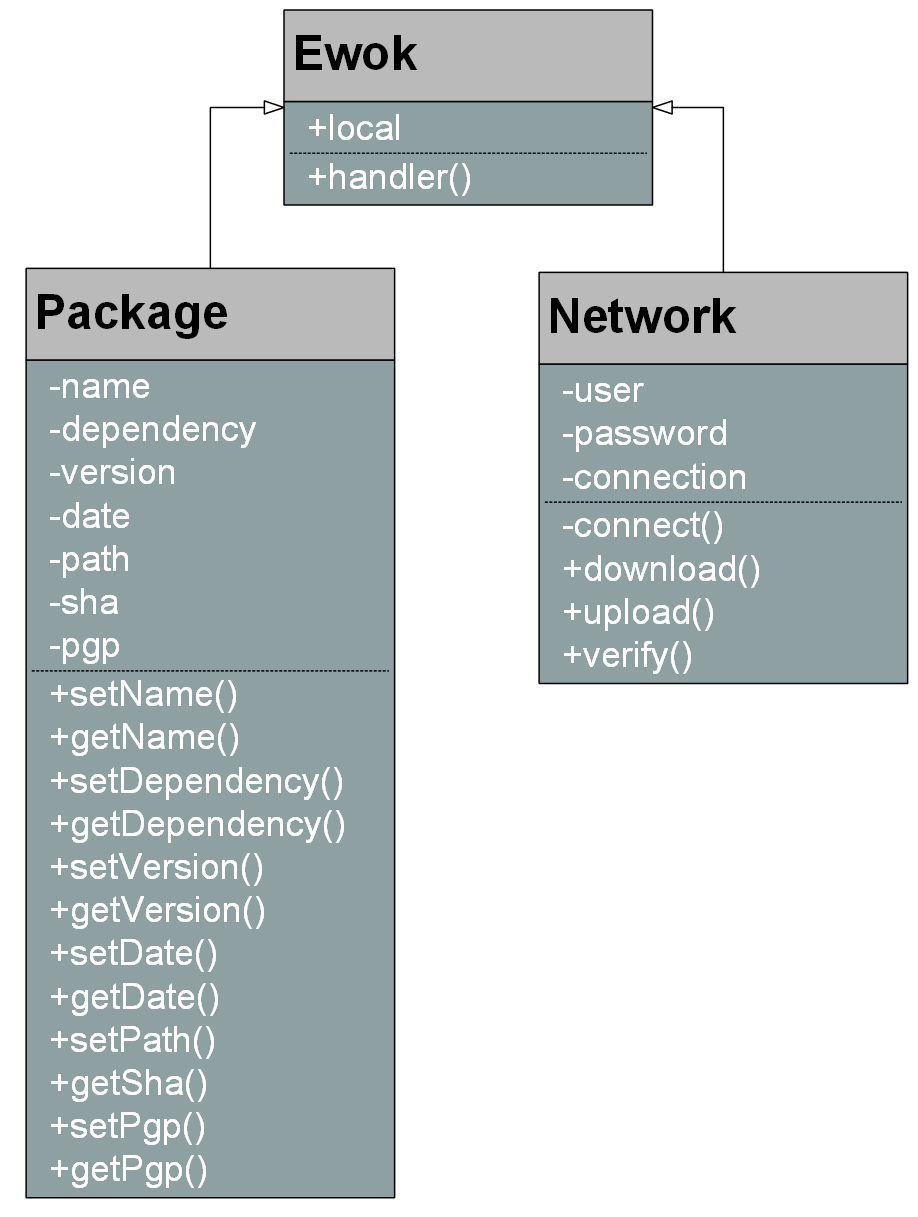
\includegraphics[width=0.8\linewidth,clip=]{./img/Img2.jpg}%
\label{fig:altes_Klassendiagramm}%
\end{minipage}
\\[\intextsep]


\section{neues Klassendiagramm}
\\[\intextsep]
\begin{minipage}{\linewidth}
\centering%
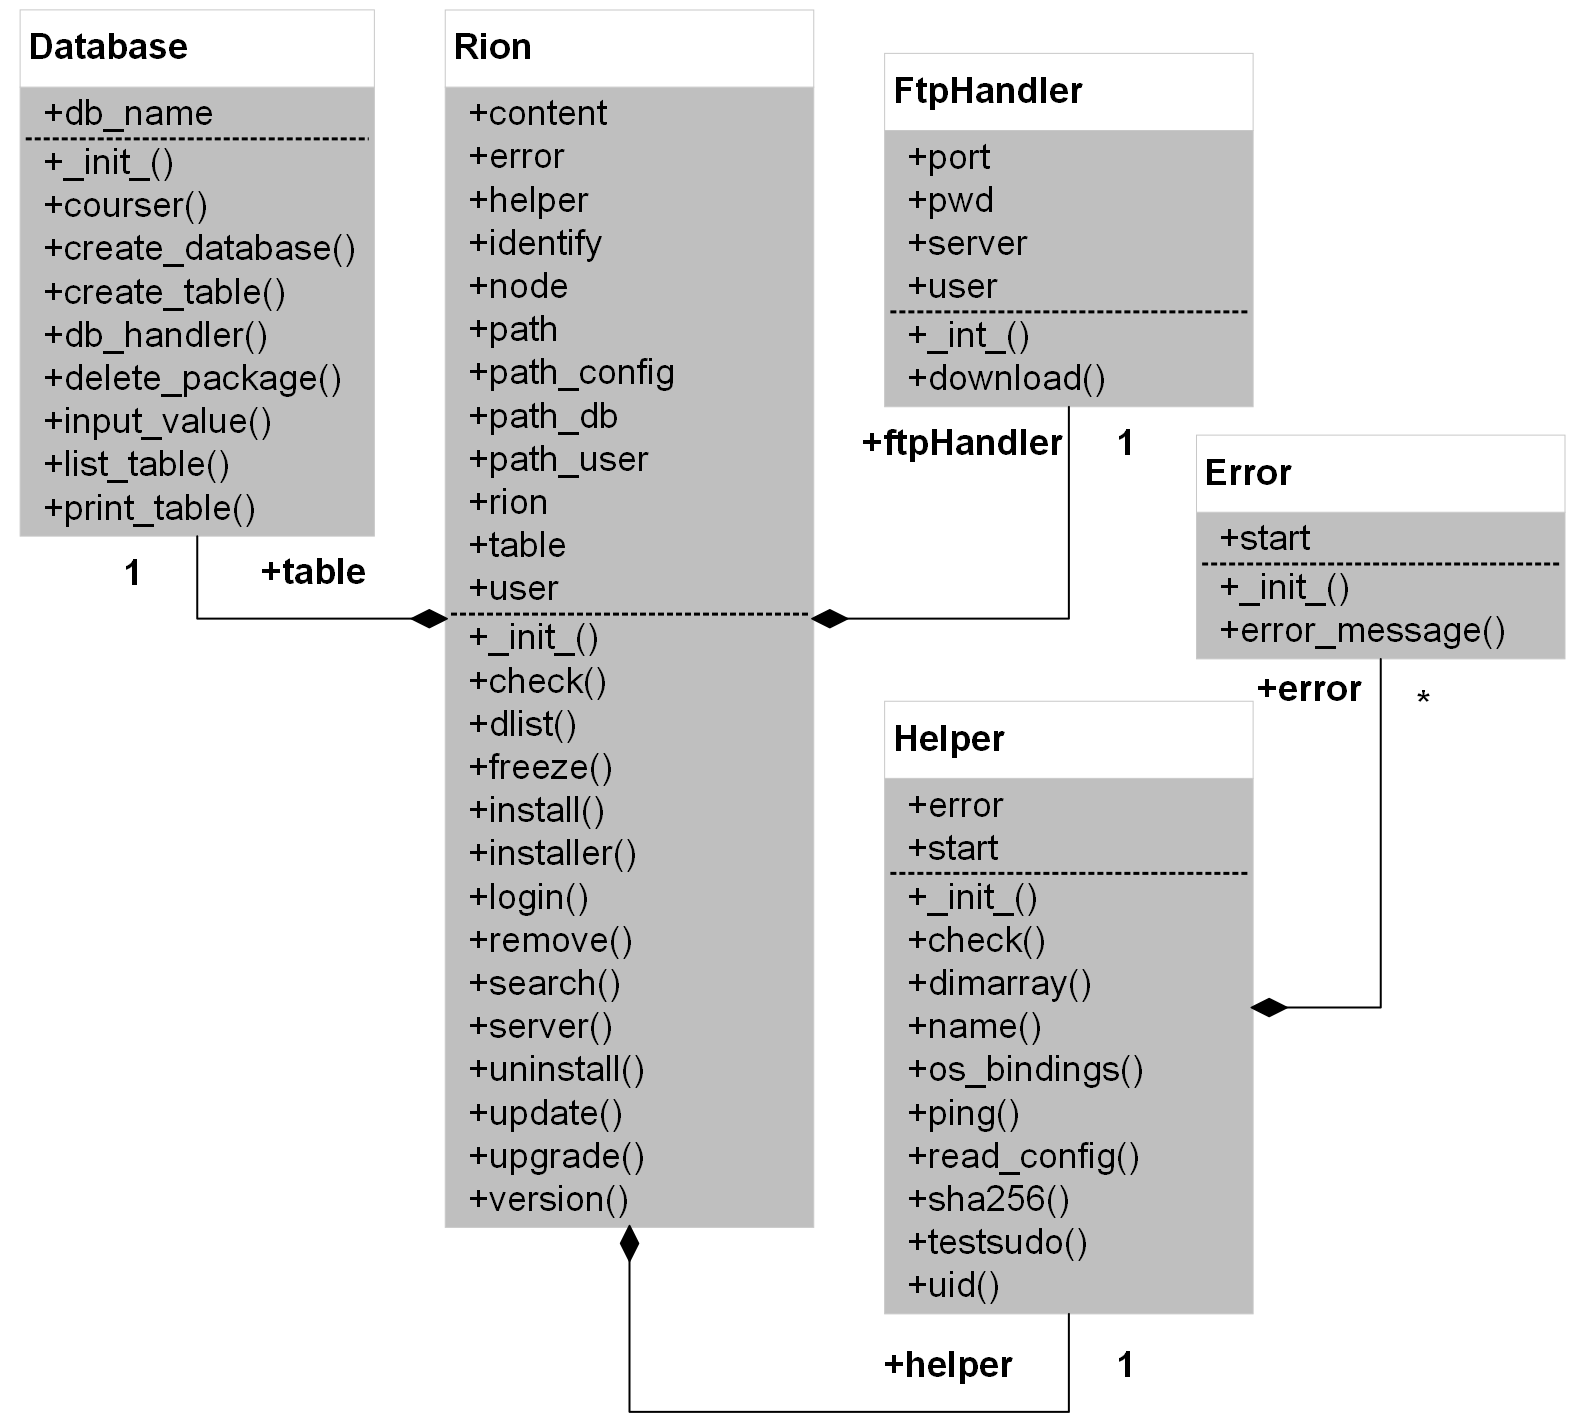
\includegraphics[width=0.8\linewidth,clip=]{./img/Img3.jpg}%
\label{fig:altes_Klassendiagramm}%
\end{minipage}
\\[\intextsep]

Aufgrund technischer Notwendigkeit mussten wir während Implementierungsphase vom
Alten auf eine Realisierung des neuen Klassendiagramms umsteigen.
    
    
\section{Sequenzdiagramm}
\\[\intextsep]
\begin{minipage}{\linewidth}
\centering%
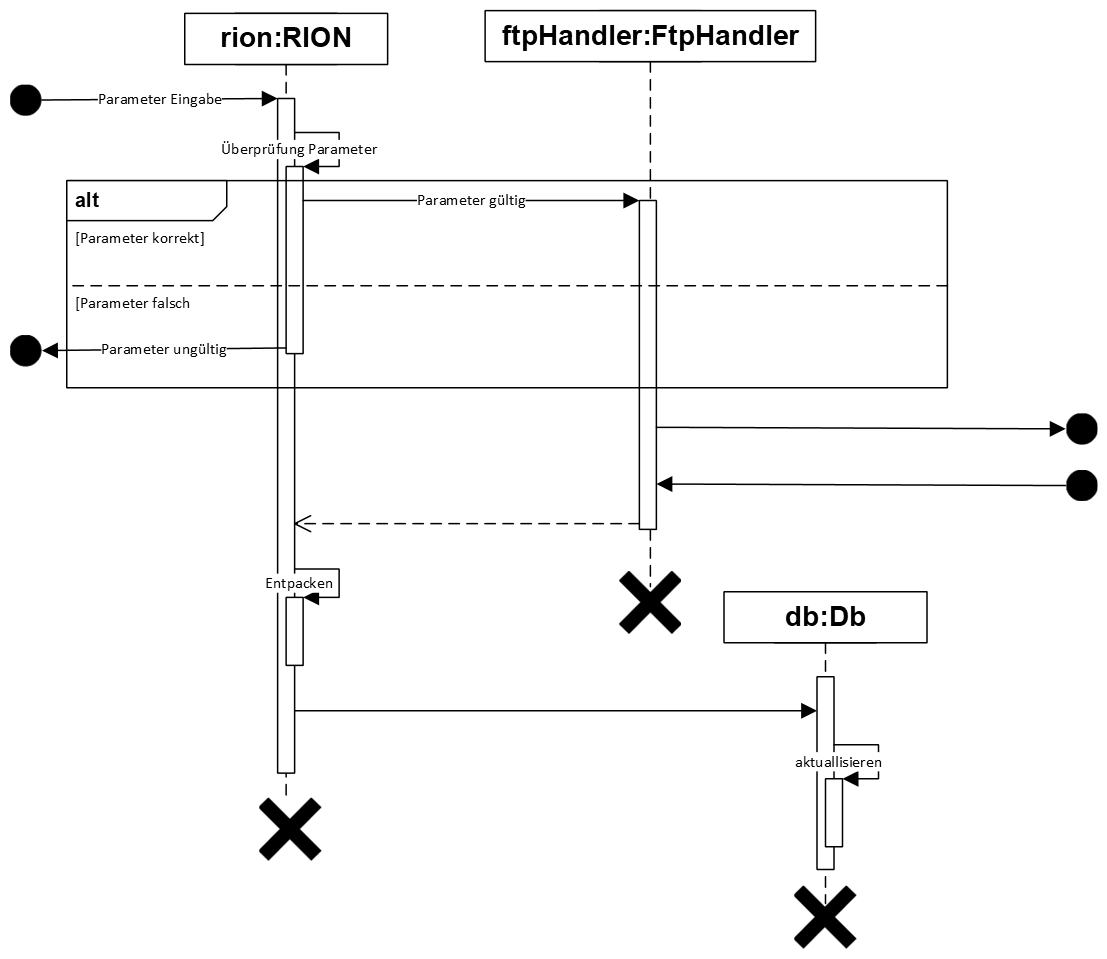
\includegraphics[width=0.8\linewidth,clip=]{./img/Img4.jpg}%
\label{fig:altes_Klassendiagramm}%
\end{minipage}
\\[\intextsep]
\clearpage

Entscheidung 1\\
Aufgabe: Protokoll mit dem Rion auf die Pakete des Servers zugreift\\

Ursprünglich war geplant, Rion und INOR via Client-Server-Modell eng miteinader zu
verknüpfen. In der eigentlichen Implemetierung stellte sich jedoch heraus, dass ein
klassischer Ansatz sinnvoller ist: \\

Inor arbeitet unabhängig von Rion. Seine Aufgabe besteht allein darin, Ordner mit Paketen
bzw. physichen Links auf Pakete zu befüllen. Auf diese wird dann mittels eines Protokolls
zugegriffen. Hierfür gibt es primär zwei verschlüsselte Optionen:\\

\begin{itemize}
    \item Option 1: https
    \begin{itemize}
        \item Vorteile:
            \begin{itemize}
                \item beste Übertragungsgescheindigkeit
            \end{itemize}
        \item Nachteile:
            \begin{itemize}
                \item  Arbeitet nicht direkt auf Dateienebene
                \item Aufwendige Impelmentierung der Authentifikation
            \end{itemize}
    \end{itemize}
     \item Option 2: ftps
    \begin{itemize}
        \item Vorteile
        \begin{itemize}
        \item Arbeitet direkt auf der Dateienebene
        \item pyftpflib bietet bereits eine ausgereifte und gut getestete Implemtierung zur
Authentifikation in Form von virtuellen Nutzern
        \end{itemize}
        \item Nachteile
        \begin{itemize}
            \item Nicht die beste, aber immernoch eine sehr gute Geschwindigkeit
        \end{itemize}
        Konklusion: Aufgrund der Möglichkeit virtuelle Nutzer anzulegen, ist ftps aus unserer Sicht
die für RION/INOR richtige Entscheidung.


        
    \end{itemize}
\end{itemize}
\clearpage

Entscheidung 2
Aufgabe: Festlegen eines Tools zur Verwaltung von installierbaren und installierten Paketen.

\begin{itemize}
    \item Option 1: Sqlite3
    \begin{itemize}
        \item Vorteile
        \begin{itemize}
            \item native Einbindung
            \item komplexer Anfragen funktionieren einfacher
            \item leichtgewichtigt
        \end{itemize}
        \item Nachteile
            \item Nicht ohne entsprechendes Programm lesba
            \item Entsprechende Binarys für jede Plattform
    \end{itemize}
     \item Option 2: json  
    \begin{itemize}
        \item Vorteile
        \begin{itemize}
            \item leichtgewichtiger
            \item plain text
        \end{itemize}
    \end{itemize}
\end{itemize}

Konklusion: Sqlite3 mag den Nachteil haben, dass es normalerweise eine systemspezifische
Binary benötigt, dies wird jedoch durch die Einbindung in Python umgangen. Dies kombiniert
mit den einfachen Möglichkeiten für komplexe Anfragen, hat den Ausschlag für Sqlite3
gegeben

    